\subsection{Sviluppo}

\subsubsection{Introduzione}
L'ISO/IEC 12207:1995 stabilisce le linee guida per il processo di sviluppo, il quale include attività cruciali come analisi, progettazione, codifica, integrazione, testing, installazione e accettazione. È fondamentale svolgere queste attività in stretta aderenza alle linee guida e ai requisiti definiti nel contratto con il cliente, garantendo così un'implementazione accurata e conforme alle specifiche richieste.

\subsubsection{Analisi dei requisiti}
L'analisi dei requisiti è una attività critica nello sviluppo del software, poiché stabilisce le basi per il design, l'implementazione e i test del sistema. Secondo lo standard ISO/IEC 12207:1995, lo scopo dell'analisi dei requisiti è di comprendere e definire in modo esaustivo le esigenze del cliente e del sistema. \\
L’attività di analisi richiede di rispondere a domande fondamentali come: “Qual è il dominio?”, “Qual è la cosa giusta da fare?” e consiste nella comprensione approfondita del dominio e nella definizione chiara di obiettivi, vincoli e requisiti sia tecnici che funzionali
\paragraph{Obbiettivi:}
\begin{itemize}
    \item Definire insieme al proponente gli obiettivi del prodotto per rispecchiarne le aspettative, comprendendo l'identificazione, documentazione e validazione dei requisiti funzionali e non funzionali;
    \item Facilitare la comprensione comune tra gli stakeholder e il team di sviluppo;
    \item Permettere una stima sulle tempistiche e sui costi;
    \item Fornire ai progettisti requisiti chiari e di facile comprensione;
    \item Favorire l'attività di verifica e test fornendo dei riferimenti pratici.
\end{itemize}

\paragraph{Documentazione}
È compito degli analisti effettuare l'Analisi dei Requisiti, redigendo un documento con il
medesimo nome che deve contenere:
\begin{itemize}
    \item Introduzione: Scopo del documento stesso;
    \item Descrizione: Analisi del prodotto
          \begin{itemize}
              \item Obbiettivi del prodotto;
              \item Funzionalità del prodotto;
              \item Caratteristiche utente;
              \item Tecnologie.
          \end{itemize}
    \item  Casi d'uso: Funzionalità offerte dal sistema dal punto di vista dell'utente
        \begin{itemize}
            \item Attori: Utenti esterni al sistema;
            \item Elenco dei casi d'uso:
            \begin{itemize}
                \item Casi d'uso in formato testuale;
                \item Diagrammi dei casi d'uso.
            \end{itemize}  
        \end{itemize}
    \item Requisiti:
        \begin{itemize}
            \item Requisiti funzionali;
            \item Requisiti qualitativi;
            \item Requisiti di vincolo.
        \end{itemize}
\end{itemize}
\paragraph{Casi d'uso}
Forniscono una descrizione dettagliata delle funzionalità del sistema dal punto di vista degli utenti, identificando come il sistema risponde a determinate azioni o scenari. In breve, i casi d'uso sono strumenti utilizzati nell'analisi dei requisiti per catturare e illustrare in modo chiaro e comprensibile come gli utenti interagiranno con il software e quali saranno i risultati di tali interazioni. \\
Ogni caso d'uso e costituito da:
\begin{enumerate}
    \item \textbf{Identificativo} nel formato:\\
          \begin{center}
              \textbf{UC [Numero caso d'uso] . [Numero sotto caso d'uso] - [Titolo]}
          \end{center}
          (ex. UC6.1 - Visualizzazione posizione sensore).\\
          con:
          \begin{itemize}
              \item \textbf{Numero caso d'uso:} ID numerico del caso d'uso;
              \item \textbf{Numero sotto caso d'uso:} ID numerico del sottocaso d'uso, presente esclusivamente in caso di presenza di un sottocaso d'uso.
              \item \textbf{Titolo}: Titolo breve ed esplicativo del caso d'uso.
          \end{itemize}
    \item \textbf{Attore principale:} Entità esterna che interagisce attivamente con il sistema per soddisfare una sua necessità;
    \item \textbf{Attore secondario:} Eventuale entità esterna che non interagisce attivamente con il sistema, ma all'interno di un caso d'uso permette al sistema di soddisfare il bisogno dell'attore principale.
    \item \textbf{Descrizione:} Eventuale descrizione breve della funzionalità;
    \item \textbf{Scenario principale:} Sequenza di eventi che si verificano quando un attore interagisce con il sistema per raggiungere l'obbiettivo del caso d'uso (Postcondizioni);
    \item \textbf{Estensioni:} Scenari alternativi (se presenti) che, in seguito ad una o più specifiche condizioni, portano il flusso del caso d'uso a non giungere alle Postcondizioni (Opzionale);
    \item \textbf{Precondizioni:} Stato in cui si deve trovare il sistema affinché la funzionalità sia disponibile all'attore;
    \item \textbf{Postcondizioni:} Stato in cui si trova il sistema dopo l'esecuzione dello scenario principale;
    \item \textbf{User story associata:} Breve descrizione di una funzionalità del software, scritta dal punto di vista dell'utente, che fornisce contesto, obiettivi e valore. \\
    Nella forma: "Come [utente] desidero poter [funzionalita] per [valore aggiunto].
\end{enumerate}

\paragraph{Diagrammi dei casi d'uso} \todo{tutte le immagini sono da ridimensionare bene e forse aggiungerei degli spazi dopo le caption e prima dell'item successivo}
I diagrammi dei casi d'uso sono strumenti grafici che permettono di visualizzare in modo chiaro e intuitivo le funzionalità offerte dal sistema dal punto di vista dell'utente. Inoltre, consentono di identificare e comprendere rapidamente le relazioni e le interazioni tra i vari casi d'uso, offrendo una visione d'insieme delle dinamiche del sistema.\\
I diagrammi dei casi d'uso si concentrano sulla descrizione delle funzionalità del sistema dal punto di vista degli utenti senza approfondire dettagli implementativi. La loro finalità principale è evidenziare le interazioni esterne al sistema, offrendo una visione focalizzata sulle funzionalità e sull'interazione dell'utente con il sistema stesso.
Un diagramma dei casi d'uso fornisce una panoramica visuale delle interazioni chiave tra gli attori e il sistema, facilitando la comprensione dei requisiti funzionali del sistema e la comunicazione tra gli stakeholder del progetto.
Di seguito sono elencati i principali componenti di un diagramma dei casi d'uso:

\begin{itemize}
    \item \textbf{Attori:}
    Gli attori sono le entità esterne al sistema che interagiscono con esso e possono essere utenti umani, altri sistemi software o componenti esterne. \\
    Gli attori sono rappresentati come "stickman" all'esterno del rettangolo che delinea il sistema.
    \begin{minipage}[t]{\linewidth}
        \centering
        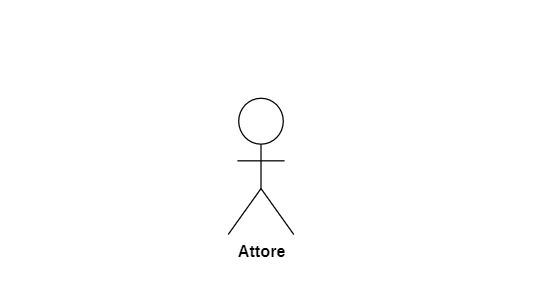
\includegraphics[width=0.6\textwidth]{../Images/NormeDiProgetto/Attore.PNG}
        \captionof{figure}{Rappresentazione Attore}
    \end{minipage}

    \item \textbf{Casi d'Uso:}
    I casi d'uso identificano le diverse funzionalità offerte dal sistema con cui l'attore può interagire. \\
    Ogni caso d'uso viene rappresentato tramite una forma ovale contenente un ID ed un titolo esplicativo.
    \begin{minipage}[t]{\linewidth}
        \centering
        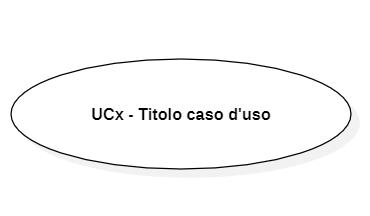
\includegraphics[width=0.6\textwidth]{../Images/NormeDiProgetto/UC.PNG}
        \captionof{figure}{Rappresentazione caso d'uso}
    \end{minipage}

    \item \textbf{Sottocasi d'uso:}
    Un sottocaso d'uso rappresenta una versione più dettagliata di un caso d'uso più generico, offrendo un livello di dettaglio più approfondito sulle funzionalità o sui particolari scenari di utilizzo rispetto al caso d'uso principale.
    \begin{minipage}[t]{\linewidth}
        \centering
        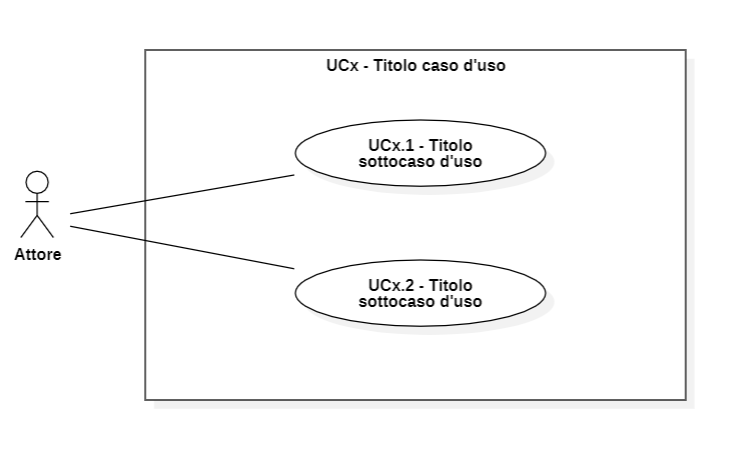
\includegraphics[width=0.6\textwidth]{../Images/NormeDiProgetto/SottocasoD'Uso.PNG}
        \captionof{figure}{Rappresentazione sottocaso d'uso}
    \end{minipage}

    \item \textbf{Sistema:}
    Il sistema viene rappresentato da un rettangolo e viene identificato con un titolo. All'interno del sistema saranno collocati i casi d'uso, mentre al suo esterno gli attori.
    \begin{minipage}[t]{\linewidth}
        \centering
        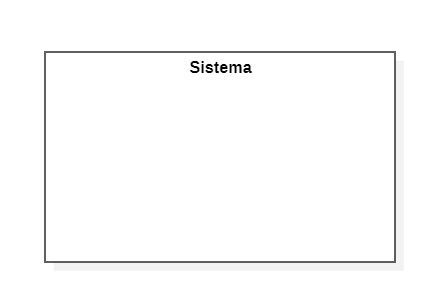
\includegraphics[width=0.6\textwidth]{../Images/NormeDiProgetto/Sistema.PNG}
        \captionof{figure}{Rappresentazione sistema}
    \end{minipage}

    \item \textbf{Relazioni tra Attori e Casi d'Uso:}
    \begin{itemize}
        \item \textbf{Associazione:}
        Le linee di associazione collegano gli attori ai casi d'uso corrispondenti, indicando quali attori sono coinvolti in una particolare interazione. Più precisamente, una linea di associazione collega un attore a un caso d'uso quando quell'attore è coinvolto nell'interazione descritta dal caso d'uso stesso. Questo legame rappresenta visivamente il ruolo dell'attore nell'utilizzo o nell'avvio di una funzione specifica offerta dal sistema.
        \begin{minipage}[t]{\linewidth}
            \centering
            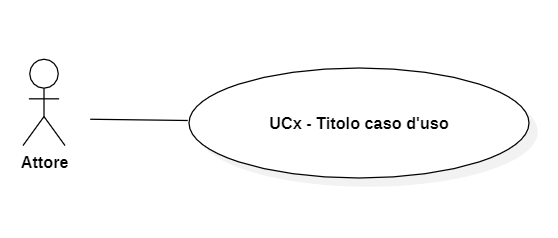
\includegraphics[width=0.6\textwidth]{../Images/NormeDiProgetto/Associazione.PNG}
            \captionof{figure}{Rappresentazione associazione}
        \end{minipage}
    \end{itemize}

    \item \textbf{Relazioni tra attori:}
    \begin{itemize}
        \item \textbf{Generalizzazione tra attori:}
        La generalizzazione tra attori rappresenta una relazione di ereditarietà tra attori, dove un attore specializzato (figlio) eredita comportamenti e caratteristiche da un attore base (genitore). Questo aiuta a organizzare gerarchicamente gli attori coinvolti nell'interazione con il sistema nei diagrammi dei casi d'uso.
        \begin{minipage}[t]{\linewidth}
            \centering
            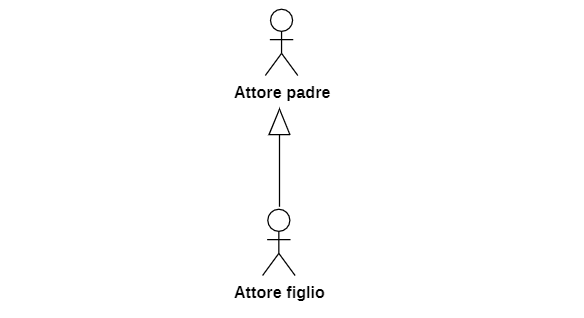
\includegraphics[width=0.6\textwidth]{../Images/NormeDiProgetto/GeneralizzazioneAttori.PNG}
            \captionof{figure}{Rappresentazione generalizzazione tra attori}
        \end{minipage}
    \end{itemize}
    
    \item \textbf{Relazioni tra casi d'uso:}
    \begin{itemize}
        \item \textbf{Inclusione:}
        La relazione di inclusione indica che un caso d'uso (detto "includente") include il comportamento di un altro caso d'uso (detto "incluso"). In pratica, quando un attore avvia il caso d'uso includente, il caso d'uso incluso viene eseguito come parte integrante del primo. Questo è utile per evitare la duplicazione del codice o delle azioni in diversi casi d'uso. La relazione di inclusione è spesso rappresentata da una freccia con la punta aperta.
        Esempio: Supponiamo che ci sia un caso d'uso generico chiamato "Autenticazione". Questo caso d'uso può includere il caso d'uso più specifico "Gestione Password". Quando un utente si autentica, il sistema eseguirà anche la gestione della password come parte del processo di autenticazione.
        \begin{minipage}[t]{\linewidth}
            \centering
            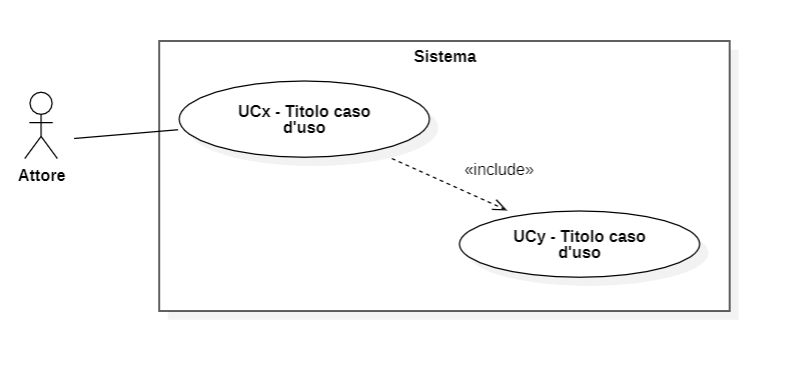
\includegraphics[width=0.6\textwidth]{../Images/NormeDiProgetto/Inclusione.PNG}
            \captionof{figure}{Rappresentazione inclusione}
        \end{minipage}

        \item \textbf{Estensione:}
        La relazione di estensione indica che un caso d'uso (detto "estendente") può estendere il comportamento di un altro caso d'uso (detto "esteso") in determinate circostanze. In altre parole, l'esecuzione del caso d'uso estendente può essere condizionalmente estesa o arricchita dal caso d'uso esteso. La relazione di estensione è spesso rappresentata da una freccia con la punta chiusa.
        Esempio: Considera un caso d'uso "Gestione Ordini". Questo caso d'uso potrebbe estendere il caso d'uso "Verifica Disponibilità" se durante la gestione degli ordini si verifica la necessità di verificare la disponibilità di un determinato prodotto. In questo modo, l'estensione permette di gestire situazioni specifiche senza ingombrare il flusso principale del caso d'uso base.
        \begin{minipage}[t]{\linewidth}
            \centering
            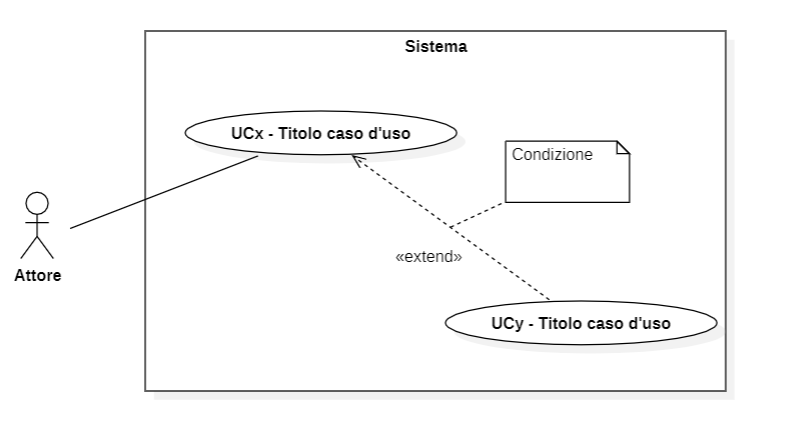
\includegraphics[width=0.6\textwidth]{../Images/NormeDiProgetto/Estensione.PNG}
            \captionof{figure}{Rappresentazione estensione}
        \end{minipage}

        \item \textbf{Generalizzazione casi d'uso:}
        La generalizzazione nei diagrammi dei casi d'uso rappresenta una relazione di ereditarietà tra casi d'uso, indicando che un caso d'uso più specifico eredita il comportamento da un caso d'uso più generico. Questa relazione è simboleggiata da una linea con una freccia vuota che punta dal caso d'uso più specifico al caso d'uso più generico.
        \begin{minipage}[t]{\linewidth}
            \centering
            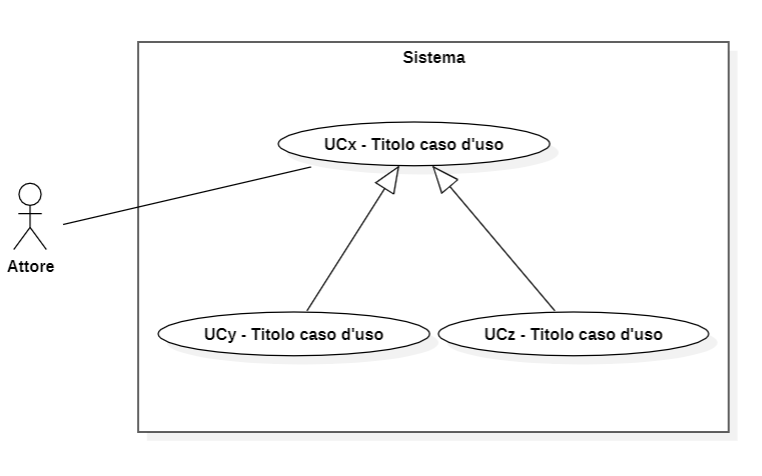
\includegraphics[width=0.6\textwidth]{../Images/NormeDiProgetto/GeneralizzazioneUC.PNG}
            \captionof{figure}{Rappresentazione generalizzazione}
        \end{minipage}
    \end{itemize}

\end{itemize}

\paragraph{Requisiti}
I requisiti di un prodotto software sono specifiche dettagliate e documentate che delineano le funzionalità, le prestazioni, i vincoli e altri aspetti critici che il software deve soddisfare. Questi requisiti fungono da guida per lo sviluppo, il testing e la valutazione del prodotto, assicurando che risponda alle esigenze degli utenti e agli obiettivi del progetto.
Includono
\begin{itemize}
    \item \textbf{Requisiti funzionali:} Descrivono le funzionalità che il software deve avere.
    \item \textbf{Requisiti non funzionali:} Definiscono principalmente criteri di prestazione, qualità, sicurezza e vincoli del sistema, ovvero caratteristiche che non riguardano direttamente le funzionalità specifiche del software.
\end{itemize}
Una precisa definizione dei requisiti è fondamentale: devono risultare inequivocabili e rispondere pienamente alle attese del cliente o del proponente.\\
Ogni requisito è costituito da:
\begin{enumerate}
    \item \textbf{Identificativo} nel formato:\\
          \begin{center}
              \textbf{R [Abbreviazione tipologia requisito] [Codice]}
          \end{center}
          con:
          \begin{itemize}
              \item \textbf{Abbreviazione tipologia requisito:}
                    \begin{itemize}
                        \item \textbf{RF:} Requisito funzionale;
                        \item \textbf{RQ:} Requisito qualitativo;
                        \item \textbf{RV:} Requisito di vincolo;
                    \end{itemize}
              \item \textbf{Codice:} Identificativo progressivo all'interno della tipologia di requisito.
          \end{itemize}
    \item \textbf{Importanza:}
          \begin{itemize}
              \item \textbf{Obbligatorio:} irrinunciabile per qualcuno degli stakeholder;
              \item \textbf{Desiderabile:} non strettamente necessario ma a valore aggiunto;
              \item \textbf{Opzionale:} relativamente utile o contrattabile più avanti nel tempo.
          \end{itemize}
    \item \textbf{Descrizione:} Narrazione chiara e dettagliata che fornisce una spiegazione completa del comportamento o della caratteristica che il software deve possedere;
    \item \textbf{Fonte:} Fonte del requisito (ex. capitolato, Verbale interno/esterno);
    \item \textbf{Casi d'uso:} Elenco casi d'uso associati.
\end{enumerate}
\paragraph{Metriche}
Le metriche nell'analisi dei requisiti sono strumenti utilizzati per valutare, misurare e gestire diversi aspetti dei requisiti di un sistema o di un progetto. Queste metriche aiutano a garantire che i requisiti siano completi, corretti, coerenti e comprensibili. Alcune metriche comuni utilizzate nell'analisi dei requisiti includono:
\begin{itemize}
    \item \textbf{Completezza dei requisiti:} Misura la quantità di requisiti identificati rispetto a quelli effettivamente necessari per il sistema. Una metrica comune è la percentuale di requisiti identificati rispetto a quelli totali;
    \item \textbf{Coerenza:} Valuta la coerenza tra i requisiti. Ad esempio, si potrebbe misurare il numero di conflitti o di requisiti duplicati;
    \item \textbf{Tracciabilità:} Indica la capacità di tracciare i requisiti attraverso le fasi del progetto. Si possono usare metriche come il numero di requisiti tracciati rispetto al totale;
    \item \textbf{Comprensibilità:} Misura la chiarezza e la comprensibilità dei requisiti. Si potrebbe valutare tramite sondaggi o questionari la facilità con cui gli stakeholder comprendono i requisiti;
    \item \textbf{Stabilità:} Misura quanto i requisiti cambiano nel tempo. Si possono usare metriche come il tasso di cambiamento dei requisiti per periodo;
    \item \textbf{Priorità:} Valuta l'importanza relativa dei requisiti. Si possono assegnare punteggi di priorità ai requisiti e valutare la distribuzione di questi punteggi;
    \item \textbf{Testabilità:} Misura la facilità con cui i requisiti possono essere verificati tramite test. Si potrebbe valutare la quantità di requisiti che possono essere testati e quelli che richiedono ulteriori specifiche per la verifica;
    \item \textbf{Misurazione del rischio:} Valuta il livello di rischio associato ai requisiti. Si potrebbero utilizzare valutazioni qualitative o quantitative per attribuire livelli di rischio a ciascun requisito.
\end{itemize}
Ognuna di queste metriche è necessaria ad assicurare che i requisiti siano gestiti in modo efficace e che siano allineati alle esigenze degli stakeholder.

\paragraph{Strumenti} \todo{da inserire}

\subsubsection{Progettazione}

\paragraph{Scopo}
La finalità dell'attività di progettazione è quella di identificare una soluzione realizzativa adeguata in grado di soddisfare appieno le esigenze di tutti gli stakeholder, tenendo conto dei requisiti e delle risorse disponibili. \\
L'attività di progettazione risponde alla domanda fondamentale: "Come fare la cosa giusta relativamente a quello di cui c’è bisogno?" \\
È fondamentale definire l'architettura del prodotto prima di avviare la fase di codifica perseguendo correttezza per costruzione piuttosto che correttezza per correzione e in modo tale da gestire in modo efficiente la complessità del prodotto, garantendo una struttura solida e coerente durante tutto il processo di sviluppo.

\paragraph{Obiettivi}
La definizione di un'architettura solida è fondamentale per il successo del progetto. \\
L'obiettivo è garantire il soddisfacimento dei requisiti attraverso un sistema di qualità definito dall'architettura del prodotto. \\
Ciò comporta:
\begin{itemize}
    \item Identificazione di parti componibili conformi ai requisiti con specifiche chiare e coese, realizzandole con risorse sostenibili e costi contenuti;
    \item Organizzazione del sistema atto ad agevolare futuri adattamenti;
    \item Gestione della complessità del sistema attraverso una progettazione dettagliata, suddividendo il sistema in unità architetturali per rendere la codifica di ogni singola parte facilmente gestibile, rapida e verificabile.
\end{itemize}
L'output della fase di progettazione software consiste in diversi artefatti e documenti che forniscono una guida dettagliata per lo sviluppo del sistema. \\
Questi output includono:
\begin{itemize}
    \item \textbf{Documenti di progettazione:} Raccolgono informazioni dettagliate sull'architettura del sistema, la struttura dei dati, i moduli e i componenti del software. Questi documenti descrivono come il sistema sarà realizzato e come i vari elementi interagiranno tra di loro;
    \item \textbf{Diagrammi UML:} Offrono rappresentazioni visive dell'architettura e del design del sistema. Questi diagrammi possono includere diagrammi delle classi, diagrammi dei casi d'uso, diagrammi di sequenza, diagrammi di attività e altri, fornendo una visione chiara e strutturata dei diversi aspetti del software;
    \item \textbf{Specifiche dei componenti e delle interfacce:} Descrivono in dettaglio i singoli componenti del sistema, specificando le loro funzionalità, interfacce, requisiti di input e output, così come le relazioni con altri componenti.
    \item \textbf{Design Patterns e Best Practices:} Se necessario, vengono identificati e documentati i design patterns e le best practices utilizzate nel progetto per garantire coerenza, efficienza e manutenibilità del codice;
    \item \textbf{Prototipi e modelli:} In alcuni casi, vengono creati prototipi o modelli parziali del sistema per testare e verificare il design iniziale, permettendo di raccogliere feedback e apportare modifiche prima della fase di sviluppo completa;
    \item \textbf{Piani di test di progettazione:} Definiscono i criteri e le strategie per testare la correttezza e l'efficacia del design. Questi piani di test aiutano a verificare che il design si comporti come previsto e soddisfi i requisiti specificati.
\end{itemize}
Questi output rappresentano la base fondamentale per gli sviluppatori durante la fase di implementazione, fornendo istruzioni chiare e dettagliate su come costruire il software in conformità con i requisiti stabiliti e il design concettuale delineato.

\paragraph{Documentazione}
Ogni Baseline sarà accompagnata dalla redazione di documentazione relativa:
\begin{itemize}
    \item Technology Baseline
    \begin{itemize}
        \item Proof of concept
        \item Definizione delle componenti
        \item Scelte tecnologiche
    \end{itemize}
    \item Product Baseline
    \begin{itemize}
        \item Diagrammi UML
        \item Design pattern
        \item Definizione delle classi
        \item Test unitari
    \end{itemize}
\end{itemize}

\paragraph{Aspettative}

\paragraph{Diagrammi UML}
Vantaggi:
\begin{itemize}
    \item \textbf{Chiarezza nella comunicazione:} Rendono più comprensibili e chiari i concetti tecnici ai team e agli stakeholder;
    \item \textbf{Standardizzazione:} Offrono un linguaggio comune per la documentazione e la comprensione dei sistemi software;
    \item \textbf{Analisi e progettazione visiva:} Aiutano a identificare errori e lacune nel progetto prima dell'implementazione;
    \item \textbf{Modellazione e simulazione:} Consentono la creazione di modelli predittivi, riducendo rischi e costi durante lo sviluppo;
    \item \textbf{Facilitano la manutenzione:} Semplificano la comprensione della struttura del software, agevolando le operazioni di manutenzione;
    \item \textbf{Riducono errori di progettazione:} Aiutano a individuare problemi prima dell'implementazione, riducendo correzioni costose;
    \item \textbf{Supportano la documentazione:} Offrono una guida visiva per comprendere il sistema, inclusa nella documentazione del progetto.
\end{itemize}

\paragraph{Metriche}

\paragraph{Strumenti}
\begin{itemize}
    \item \textbf{StarUML:} \todo{forse andrebbe anche sopra, negli strumenti dell'analisi dei requisiti}
    È un'applicazione software utilizzata per creare diagrammi e modelli UML nel processo di sviluppo del software. \\
    Aiuta a visualizzare graficamente i vari aspetti di un sistema, consentendo agli utenti di creare e modificare facilmente diagrammi UML come diagrammi dei casi d'uso, delle classi, di attività e altri, semplificando così il processo di progettazione e analisi dei sistemi software.
\end{itemize}

\subsubsection{Codifica}
\paragraph{Scopo}
L'attività di codifica è affidata al programmatore e rappresenta il momento cruciale in cui le funzionalità richieste dal proponente prendono forma. \\
Durante questa fase, le idee e i concetti delineati dai progettisti vengono tradotti in codice, creando istruzioni e procedure che i calcolatori possono eseguire. \\
I programmatori devono rispettare scrupolosamente le linee guida e le norme stabilite per garantire che il codice sia in linea con le specifiche stabilite e che traduca in modo accurato le concezioni iniziali dei progettisti.
\paragraph{Aspettative}
La codifica è finalizzata alla creazione di un prodotto software in linea con le richieste del committente e conforme agli accordi stipulati.\\
Il rigoroso rispetto delle norme garantisce la creazione di codice di alta qualità, facilitando la manutenzione, l'estensione e la verifica del software, contribuendo costantemente al miglioramento della sua qualità complessiva.
\paragraph{Norme di codifica}
Le seguenti norme sono state formalizzate prendendo spunto dal libro "Clean Code" di Robert C. Martin.

\paragraph*{Nomi significativi}
Usare nomi che riflettano il significato e lo scopo delle variabili, funzioni e classi. Evitare abbreviazioni ambigue.
\paragraph*{Indentazioni e formattazione consistente}
L'utilizzo di un tab per ciascun livello di annidamento è fondamentale per assicurare una struttura coerente del codice, migliorandone la comprensione e agevolandone la gestione.
\paragraph*{Lunghezza dei metodi}
La lunghezza ottimale dei metodi può variare a seconda del contesto e delle best practices di programmazione. Tuttavia, in generale, molti esperti consigliano che i metodi siano brevi e focalizzati su una singola responsabilità.
Un principio comune è quello espresso da Robert C. Martin nel suo libro "Clean Code", che suggerisce che i metodi dovrebbero essere idealmente lunghi quanto basta per svolgere una singola operazione e non più lungo di quanto si possa visualizzare senza dover scorrere la pagina. \\
Questo favorisce:
\begin{itemize}
    \item \textbf{Chiarezza};
    \item \textbf{Manutenibilità};
    \item \textbf{Comprensibilità};
    \item \textbf{Testabilità:} Metodi più brevi sono più facili da testare in isolamento, il che favorisce l'implementazione di test di unità efficaci;
    \item \textbf{Conformità ai principi SOLID:} La brevità dei metodi è spesso correlata al principio Single Responsibility Principle (SRP) dei principi SOLID, il che favorisce la costruzione di codice più modulare e coeso.
\end{itemize} 

\paragraph*{Lunghezza righe di codice}
Mantenere le righe di codice entro i 80-120 caratteri permette una migliore leggibilità del codice su schermi di diverse dimensioni e facilita la visualizzazione di più file affiancati.
Inoltre, limitare la lunghezza delle righe può incoraggiare la scrittura di codice più chiaro e modulare.
\paragraph{Commenti}
Evitare commenti superflui e non necessari: l'obiettivo è scrivere il codice in modo chiaro e autoesplicativo, riducendo la dipendenza da commenti esplicativi. 
\subsubsection{Configurazione dell'ambiente di esecuzione}
\paragraph{Docker}

La progettazione dei Docker e la scrittura dei Dockerfile sono considerate parte del processo di sviluppo del software.
Le regole e le best practice di codifica per i file Docker sono fondamentali per garantire la creazione, la gestione e la distribuzione efficace dei container:
\begin{itemize}
    \item \textbf{Chiarezza e Coerenza:}
    \begin{itemize}
        \item Utilizzare nomi descrittivi per le immagini e i container.
        \item Mantenere una struttura coerente e consistente per assicurare un'organizzazione uniforme all'interno dei file Docker.
    \end{itemize}

\item \textbf{Versionamento:}
    \begin{itemize}
        \item Specificare sempre la versione dell'immagine di base (base image) per garantire la riproducibilità.
        \item Evitare di utilizzare tag "latest" per immagini di produzione.
    \end{itemize}

\item \textbf{Minimizzazione degli strati (Layering):}
    \begin{itemize}
        \item Ridurre il numero di istruzioni nell'esecuzione del Dockerfile per minimizzare gli strati dell'immagine.
        \item Raggruppare le istruzioni correlate per sfruttare la cache Docker.
    \end{itemize}

\item \textbf{Sicurezza:}
    \begin{itemize}
        \item Utilizzare immagini ufficiali o verificate.
        \item Evitare di eseguire processi Docker con privilegi elevati quando possibile.
        \item Usare ARG per parametrizzare informazioni sensibili.
    \end{itemize}

\item \textbf{Ottimizzazione delle risorse:}
    \begin{itemize}
        \item Limitare l'uso di risorse all'interno dei container (CPU, memoria, etc.).
        \item Usare immagini leggere e ottimizzate per la produzione.
    \end{itemize}

\item \textbf{Gestione delle variabili d'ambiente:}
    \begin{itemize}
        \item Usare variabili d'ambiente per configurazioni dinamiche.
        \item Fornire valori predefiniti opportuni per le variabili d'ambiente.
    \end{itemize}

\item \textbf{Logging e monitoraggio:}
    \begin{itemize}
        \item Configurare i container per registrare i log in modo efficace.
        \item Integrare strumenti di monitoraggio, se necessario.
    \end{itemize}

\item \textbf{Pulizia e riduzione delle dimensioni:}
    \begin{itemize}
        \item Pulire i pacchetti temporanei e le risorse non necessarie dopo l'installazione delle dipendenze.
        \item Ridurre le dimensioni delle immagini utilizzando multi-stage builds.
    \end{itemize}

\item \textbf{Documentazione:}
    \begin{itemize}
        \item Aggiungere commenti nel Dockerfile per spiegare le decisioni di progettazione.
        \item Fornire una documentazione chiara su come utilizzare e configurare il container.
    \end{itemize}

\item \textbf{Testing:}
    \begin{itemize}
        \item Implementare test automatizzati per il Dockerfile e i container, se possibile.
    \end{itemize}
\end{itemize}
\paragraph{Strumenti}
\begin{itemize}
    \item \textbf{VSCode}
    \item \textbf{Docker}
    \item \textbf{Git}
\end{itemize}
